\documentclass[12pt]{report}
\usepackage[utf8]{inputenc}
\usepackage[margin=1.2in]{geometry}
\usepackage{graphicx}
\usepackage{float}
\usepackage{subcaption}
\usepackage{amsmath}
\usepackage{amssymb}
\usepackage{ulem}
\usepackage{bm}
\usepackage{framed}
\usepackage{xcolor}
\usepackage{ragged2e}
\usepackage{color}
\usepackage{soul}
\graphicspath{ {images/} }
\setlength{\parskip}{1em}
\allowdisplaybreaks

\usepackage{titling}
\newcommand{\subtitle}[1]{%
	\posttitle{%
		\par\end{center}
	\begin{center}\large#1\end{center}
	\vskip0.5em}%
}

\newenvironment{blueframed}[1][blue]
{\def\FrameCommand{\fboxsep=\FrameSep\fcolorbox{#1}{white}}%
\MakeFramed {\advance\hsize-\width \FrameRestore}}
{\endMakeFramed}

\newenvironment{spmatrix}[1]
{\def\mysubscript{#1}\mathop\bgroup\begin{bmatrix}}
{\end{bmatrix}\egroup_{\textstyle\mathstrut\mysubscript}}

\title{Tutorial 5}
\subtitle
{
\textbf{keywords}: OLS estimator, multiple linear regression, interpretation, ceteris paribus, predict, interpretation, variation, R squared

\textbf{estimated reading time}: 30 minutes
}
\author{Quang Bui}
\date{March 26, 2018}

\begin{document}

\maketitle

\newpage
\section*{Question 1}
\underline{Multiple linear regression model and interpreting coefficients}

\noindent EViews workfile: $hprice.wf1$
\begin{figure}[H]
	\centering
	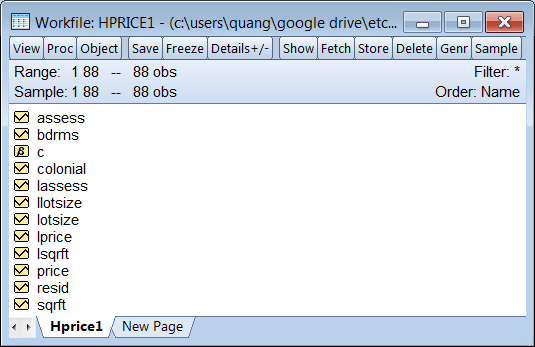
\includegraphics{q5_1}
\end{figure}
\vspace{-\baselineskip}
\noindent \textcolor{red}
{
	i. Estimate the model of $price$ on a constant, $sqrft$ and $bdrms$ and write out the results in equation form.
}
\noindent \textcolor{red}{$$price = \beta_0 + \beta_1sqrft + \beta_2bdrms + u$$ \begin{itemize}
		\item $price$ - house\ price\ (\$'000)
		\item $sqrft$ - area\ of\ the\ house\ (square foot)
		\item $bdrms$ - no.\ of\ bedrooms
\end{itemize}} \vspace{-\baselineskip}
$$Quick \to Estimate\ Equation$$
\begin{figure}[H]
	\centering
	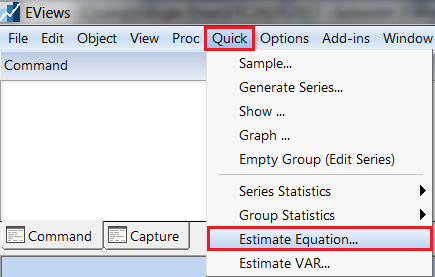
\includegraphics{q1_2}
\end{figure}
\vspace{-\baselineskip}
$$Equation\ Estimation: price\ c\ sqrft\ bdrms$$
\begin{figure}[H]
	\centering
	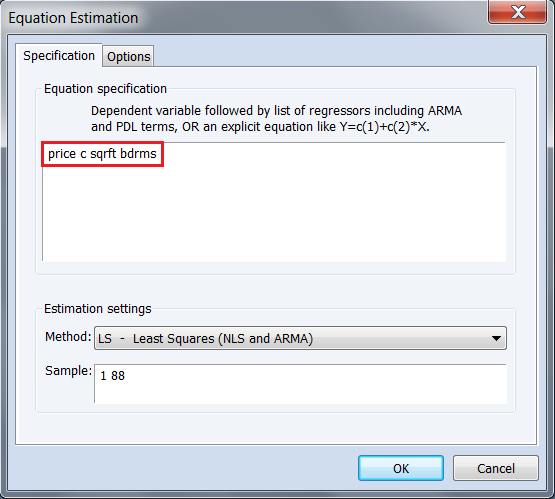
\includegraphics{q3_1}
\end{figure}
\vspace{-\baselineskip}
%%%%%%%%%% TABLE OBJECT %%%%%%%%%%
\begin{table}[H]
	\centering
	\begin{tabular}{lrrrr}
		\multicolumn{3}{l}{Dependent Variable: PRICE}&\multicolumn{1}{c}{}&\multicolumn{1}{c}{}\\
		\multicolumn{3}{l}{Method: Least Squares}&\multicolumn{1}{c}{}&\multicolumn{1}{c}{}\\
		\multicolumn{3}{l}{Date: 07/16/17   Time: 21:25}&\multicolumn{1}{c}{}&\multicolumn{1}{c}{}\\
		\multicolumn{2}{l}{Sample: 1 88}&\multicolumn{1}{c}{}&\multicolumn{1}{c}{}&\multicolumn{1}{c}{}\\
		\multicolumn{3}{l}{Included observations: 88}&\multicolumn{1}{c}{}&\multicolumn{1}{c}{}\\
		[4.5pt] \hline \\ [-4.5pt]
		\multicolumn{1}{c}{Variable}&\multicolumn{1}{r}{Coefficient}&\multicolumn{1}{r}{Std. Error}&\multicolumn{1}{r}{t-Statistic}&\multicolumn{1}{r}{Prob.}\\
		[4.5pt] \hline \\ [-4.5pt]
		\multicolumn{1}{c}{C}&\multicolumn{1}{r}{$-19.31500$}&\multicolumn{1}{r}{$31.04662$}&\multicolumn{1}{r}{$-0.622129$}&\multicolumn{1}{r}{$0.5355$}\\
		\multicolumn{1}{c}{SQRFT}&\multicolumn{1}{r}{$0.128436$}&\multicolumn{1}{r}{$0.013824$}&\multicolumn{1}{r}{$9.290506$}&\multicolumn{1}{r}{$0.0000$}\\
		\multicolumn{1}{c}{BDRMS}&\multicolumn{1}{r}{$15.19819$}&\multicolumn{1}{r}{$9.483517$}&\multicolumn{1}{r}{$1.602590$}&\multicolumn{1}{r}{$0.1127$}\\
		[4.5pt] \hline \\ [-4.5pt]
		\multicolumn{1}{l}{R-squared}&\multicolumn{1}{r}{$0.631918$}&\multicolumn{2}{l}{Mean dependent var}&\multicolumn{1}{r}{$293.5460$}\\
		\multicolumn{1}{l}{Adjusted R-squared}&\multicolumn{1}{r}{$0.623258$}&\multicolumn{2}{l}{S.D. dependent var}&\multicolumn{1}{r}{$102.7134$}\\
		\multicolumn{1}{l}{S.E. of regression}&\multicolumn{1}{r}{$63.04484$}&\multicolumn{2}{l}{Akaike info criterion}&\multicolumn{1}{r}{$11.15907$}\\
		\multicolumn{1}{l}{Sum squared resid}&\multicolumn{1}{r}{$337845.4$}&\multicolumn{2}{l}{Schwarz criterion}&\multicolumn{1}{r}{$11.24352$}\\
		\multicolumn{1}{l}{Log likelihood}&\multicolumn{1}{r}{$-487.9989$}&\multicolumn{2}{l}{Hannan-Quinn criter.}&\multicolumn{1}{r}{$11.19309$}\\
		\multicolumn{1}{l}{F-statistic}&\multicolumn{1}{r}{$72.96353$}&\multicolumn{2}{l}{Durbin-Watson stat}&\multicolumn{1}{r}{$1.858074$}\\
		\multicolumn{1}{l}{Prob(F-statistic)}&\multicolumn{1}{r}{$0.000000$}&\multicolumn{1}{c}{}&\multicolumn{1}{c}{}&\multicolumn{1}{c}{}\\
		[4.5pt] \hline \\ [-4.5pt]
	\end{tabular}
	\caption{Regression output of $price$ on a constant, $sqrft$ and $bdrms$}
	\label{tbl:regout3}
\end{table}

\vspace{-\baselineskip}
\noindent When reporting the estimated model, we must not forget to include a `hat' above the dependent variable and $se(\hat{\beta}_j)$ underneath $\hat{\beta}_j$ in parenthesis,
\begin{align*}
\widehat{price} &= \underset{(se(\hat{\beta}_0))}{\hat{\beta}_0} + \underset{(se(\hat{\beta}_1))}{\hat{\beta}_1}sqrft + \underset{(se(\hat{\beta}_2))}{\hat{\beta}_2}bdrms \\
\widehat{price} &= -\underset{(31.0466)}{19.3150} + \underset{(0.0138)}{0.1284}sqrft + \underset{(9.4835)}{15.1982}bdrms
\end{align*}
\noindent \textcolor{red}
{
	ii. What is the estimated increase in price for a house with one more bedroom, holding square footage constant?
}
\newpage
\justify
\begin{blueframed}
	\textcolor{blue}{\textbf{Background}}
	\vspace{-\baselineskip}
	\justify
	\textcolor{blue}{\underline{Interpretation of estimated coefficients for multiple linear regression models}}
	
	\noindent \textcolor{blue}
	{
		\noindent Suppose we estimate a model of $y$ on a constant, $x_1$, and $x_2$,
		$$\hat{y} = \hat{\beta}_0 + \hat{\beta}_1x_1 + \hat{\beta}_2x_2$$
		if $x_1$ and $x_2$ changes by ${\Delta}x_1$ and ${\Delta}x_2$ respectively then,
		$$x_1\ becomes\ x_1 +{\Delta}x_1$$
		$$x_2\ becomes\ x_2 +{\Delta}x_2$$
		which will change $\hat{y}$,  
		$$\hat{y}\ becomes\ \hat{y}+{\Delta}\hat{y}$$
		This then gives us the following equation,
		\begin{align*}
		\hat{y}+{\Delta}\hat{y} &= \hat{\beta}_0 + \hat{\beta}_1(x_1 + {\Delta}x_1) + \hat{\beta}_2(x_2+{\Delta}x_2) \\
		&= \hat{\beta}_0 + \hat{\beta}_1x_1 + \hat{\beta}_2x_2 + \hat{\beta}_1{\Delta}x_1 + \hat{\beta}_2{\Delta}x_2 \\
		&= \hat{y} + \hat{\beta}_1{\Delta}x_1 + \hat{\beta}_2{\Delta}x_2 
		\end{align*}
		Since $\hat{y} = \hat{\beta}_0 + \hat{\beta}_1x_1 + \hat{\beta}_2x_2$, it must follow that,
		$${\Delta}\hat{y} = \hat{\beta}_1{\Delta}x_1 + \hat{\beta}_2{\Delta}x_2$$
		$\therefore$  the change in $\hat{y}$ for a 1-unit change in $x_1$, holding $x_2$ constant, is $\hat{\beta}_1$,
		$${\Delta}x_2 = 0$$
		$${\Delta}x_1 = 1$$
		\begin{align*}
		{\Delta}\hat{y} &= \hat{\beta}_1{\Delta}x_1 + \hat{\beta}_2{\Delta}x_2 \\
		&= \hat{\beta}_1\times 1 + \hat{\beta}_2\times 0 \\
		&= \hat{\beta}_1
		\end{align*}
		and the change in $\hat{y}$ for a 1-unit change in $x_2$, holding $x_1$ constant, is $\hat{\beta}_2$,
		$${\Delta}x_2 = 1$$
		$${\Delta}x_1 = 0$$
		\begin{align*}
		{\Delta}\hat{y} &= \hat{\beta}_1{\Delta}x_1 + \hat{\beta}_2{\Delta}x_2 \\
		&= \hat{\beta}_1\times 0 + \hat{\beta}_2\times 1 \\
		&= \hat{\beta}_2
		\end{align*}
		As we can see, $\hat{\beta}_1$ and $\hat{\beta}_2$ have a partial effect (ceteris paribus) interpretation!
}\end{blueframed}

\noindent From our estimated model, the changed in estimated house price depends on the change square footage and no. of bedrooms,
$$\Delta\widehat{price} = \hat{\beta}_1\Delta sqrft + \hat{\beta}_2\Delta bdrms$$
\noindent Note: The estimated intercept coefficient does not change the estimated house price.

\noindent If square footage is held constant,
$$\Delta sqrft = 0$$
\noindent then the change in the estimated house price depends only on the change in no. of bedrooms,
\begin{align*}
\Delta\widehat{price} &= \hat{\beta}_1\Delta \times 0 + \hat{\beta}_2\Delta bdrms \\
&= \hat{\beta}_2\Delta bdrms
\end{align*}
\noindent Therefore, the estimated increase in house price for for an additional bedroom, \uline{holding square footage constant},
\begin{align*}
\Delta\widehat{price} &= \hat{\beta}_2 \times 1 \\
&= 15.1982 \times 1 \\
&= 15.1982
\end{align*}
$$\$15,198.20$$
\noindent \textcolor{red}
{
	iii. What is the estimated increase in price for a house with an additional bedroom that is 140 square feet in size? Compare this to your answer in part (ii).
}
$$\Delta bdrms = 1$$
$$\Delta sqrft = 120$$
\begin{align*}
\Delta\widehat{price} &= \hat{\beta}_1\Delta sqrft + \hat{\beta}_2\Delta bdrms \\
&= 0.1284 \times 140+15.1982 \times 1 \\
&= 33.12
\end{align*}
$$\$33,120$$
\noindent The change in estimated house price is greater here than in ii) because we are also increasing the size of the house. In ii), we estimated the change in house price for an additional bedroom but kept the size of the house the same.

\noindent \textcolor{red}
{
	iv. What percentage of the variation in price is explained by square footage and number of bedrooms?
}
$$R^2 = 63.2\%$$
\noindent 63.2\% of the variation in house price is explained by square footage and number of bedrooms.

\noindent \textcolor{red}
{
	v. The first house in the sample has $sqrft=2438$ and $bdrms=4$. Find the predicted selling price for this house from the OLS regression line.
}
\begin{align*}
\widehat{price} &= -19.3150 + 0.1284sqrft + 15.1982bdrms \\
\widehat{price}_1 &= -19.3150 + 0.1284sqrft_1 + 15.1982bdrms_1 \\
&= -19.3150+0.1284 \times 2438+15.1982 \times 4 \\
&= 354.6052
\end{align*}
$$\$354,605$$
\noindent To perform this calculation in EViews,
$$Command\ Window: scalar\ prediction\ = c(1) + c(2)^{*}2438 + c(3)^{*}4$$
\begin{figure}[H]
	\centering
	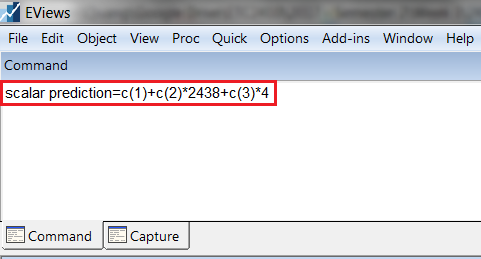
\includegraphics{q3_2}
\end{figure}
\vspace{-\baselineskip}
$$(press\ Enter\ to\ execute\ code)$$
\begin{figure}[H]
	\centering
	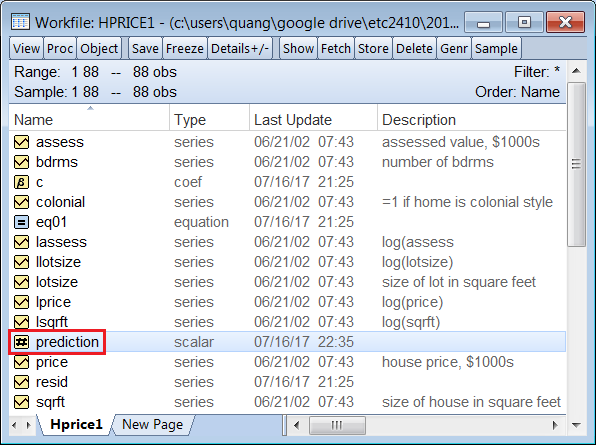
\includegraphics{q3_3}
\end{figure}
\vspace{-\baselineskip}
\begin{figure}[H]
	\centering
	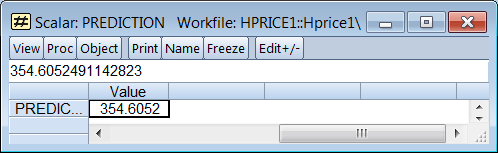
\includegraphics{q3_4}
\end{figure}

\noindent \textcolor{red}
{
	vi. The actual selling price of the first house in the sample was \$300,000 (so $price_1$=300). Find the residual for this house. Does it suggest that the buyer underpaid or overpaid for the house?
}
\begin{align*}
\hat{u}_i &= price_i - \widehat{price}_i \\
\hat{u}_1 &= price_1 - \widehat{price}_1 \\
&= 300 - 354.605 \\
&= -54.605
\end{align*}
$$-\$54,605$$
\noindent Based on our estimated model, the buyer underpaid, however, we have not considered other features that impact house price e.g. number of baths, age of house, whether it has been renovated etc.

\newpage
\section*{Question 2}
\noindent \textcolor{red}{We would like to make an ``app" where users input their easy to measure body characteristics and the app predicts their body fat percentage. We start with making an app for men. We have data on body fat percentage ($BODY\_FAT$), weight in kg ($WKG$) and abdomen circumference in cm ($ABDOMEN$) for 251 adult men. The matrix of scatter plots of each pair of these three variables in our sample is given below.}
\begin{figure}[H]
	\centering
	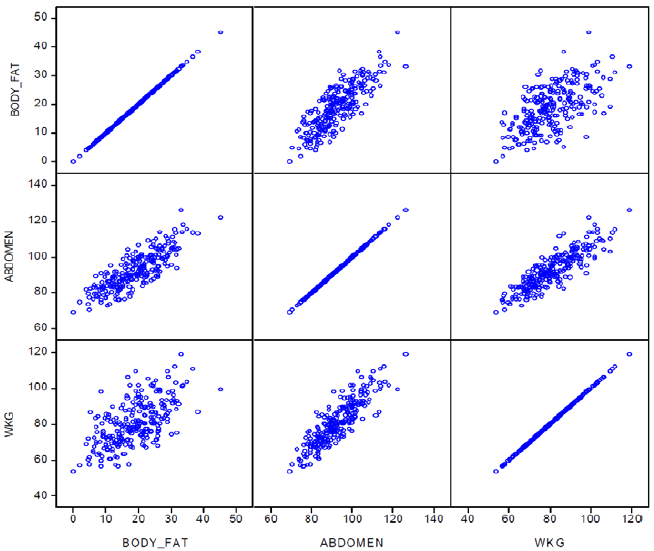
\includegraphics{tute5_28}
\end{figure}
\noindent \textcolor{red}{Without estimating any regressions, explain what these plots can tell us about each of the following (the correct answer for one of these is ``nothing"):}

\justify
\begin{blueframed}
	\textcolor{blue}{\textbf{Background}}
	\vspace{-\baselineskip}
	\justify
	\textcolor{blue}{\underline{OLS estimator for a simple linear regression model}}
	
	\noindent \textcolor{blue}
	{
		\noindent For the following simple linear regression model, 
}\end{blueframed}

\justify
\begin{blueframed}
	\noindent \textcolor{blue}
	{
		\noindent $$y = \beta_0 + \beta_1 x_1 + u$$  the OLS estimates of $\beta_0$ and $\beta_1$ can be expressed by the following formulas,
		\begin{align*}
		\hat{\beta}_0 &= \bar{y} - \hat{\beta}_1\bar{x}_1 \\
		\hat{\beta}_1 &= \dfrac{\widehat{Cov(y,x_1)}}{\widehat{Var(x_1)}}
		\end{align*}
		or in matrix notation, $$\widehat{\boldsymbol{\beta}} 
		= (\textit{\textbf{X}}'\textit{\textbf{X}})^{-1}\textit{\textbf{X}}'\textit{\textbf{y}}
		=
		\begin{bmatrix}
		\hat{\beta}_0 \\
		\hat{\beta}_1 
		\end{bmatrix}
		=
		\begin{bmatrix}
		\bar{y} - \hat{\beta}_1\bar{x}_1 \\[10pt]
		\dfrac{\widehat{Cov(y,x_1)}}{\widehat{Var(x_1)}} 
		\end{bmatrix}$$
		since $\widehat{Var(x_1)}>0$, the sign of $\hat{\beta}_1$ depends directly on the sign of $\widehat{Cov(y,x_1)}$. \\ \\ For the multiple linear regression model, $$y = \beta_0 + \beta_1 x_1 + \beta_2 x_2 + \dots + \beta_k x_k + u$$ the OLS estimate of $\beta_1$ is not equal to $\dfrac{\widehat{Cov(y,x_1)}}{\widehat{Var(x_1)}}$, $$\hat{\beta}_1 \neq \dfrac{\widehat{Cov(y,x_1)}}{\widehat{Var(x_1)}}$$ $\therefore$ the sign of $\hat{\beta}_1$, in the estimated multiple linear regression model, does not depend directly on the sign of $\widehat{Cov(y,x_1)}$.
}\end{blueframed}

\noindent \textcolor{red}{(a) the sign of the coefficient of $ABDOMEN$ in a regression of $BODY\_FAT$ on a constant and $ABDOMEN$}
\begin{align*}
BODY\_FAT &= \beta_0 + \beta_1 ABDOMEN + u \\
\widehat{BODY\_FAT} &= \hat{\beta}_0 + \hat{\beta}_1 ABDOMEN
\end{align*}
\noindent For the simple regression model of $BODY\_FAT$ on a constant and $ABDOMEN$ the OLS estimates of $\beta_0$ and $\beta_1$ are given by the following formulas,
\begin{align*}
\hat{\beta}_0 &= \overline{BODY\_FAT} - \hat{\beta}_1\overline{ABDOMEN} \\
\hat{\beta}_1 &= \dfrac{\widehat{Cov(BODY\_FAT,ABDOMEN)}}{\widehat{Var(ABDOMEN)}}
\end{align*}
\noindent From the scatter plot, we can see that $BODY\_FAT$ and $ABDOMEN$ have a positive linear relationship, 
\begin{align*}
&\therefore \widehat{Cov(BODY\_FAT,ABDOMEN)}>0 \\
&\implies \hat{\beta}_1 > 0
\end{align*}

\noindent \textcolor{red}{(b) the sign of the coefficient of $WKG$ in a regression of $BODY\_FAT$ on a constant and $WKG$}$$(different\ model\ so\ I'm\ using\ a\ different\ greek\ letter)$$
\begin{align*}
BODY\_FAT &= \alpha_0 + \alpha_1 WKG + u \\
\widehat{BODY\_FAT} &= \hat{\alpha}_0 + \hat{\alpha}_1 WKG
\end{align*}
\noindent For the simple regression model of $BODY\_FAT$ on a constant and $WKG$ the OLS estimates of $\alpha_0$ and $\alpha_1$ are given by the following formulas,
\begin{align*}
\hat{\alpha}_0 &= \overline{BODY\_FAT} - \hat{\alpha}_1\overline{WKG} \\
\hat{\alpha}_1 &= \dfrac{\widehat{Cov(BODY\_FAT,WKG)}}{\widehat{Var(WKG)}}
\end{align*}
\noindent From the scatter plot, we can see that $BODY\_FAT$ and $WKG$ have a positive linear relationship, 
\begin{align*}
&\therefore \widehat{Cov(BODY\_FAT,WKG)}>0 \\
&\implies \hat{\alpha}_1 > 0
\end{align*}

\noindent \textcolor{red}{(c) which of the two regressions explained in parts (a) and (b) is likely to have a better fit?} 
\begin{align}
\widehat{BODY\_FAT} &= \hat{\beta}_0 + \hat{\beta}_1 ABDOMEN \\
\widehat{BODY\_FAT} &= \hat{\alpha}_0 + \hat{\alpha}_1 WKG
\end{align}

\noindent The first estimated model is likely to fit the data better than the second. Why?

\noindent An OLS regression line of $(1)$ through the scatter plot of $BODY\_FAT$ against $ABDOMEN$ would have a smaller sum of squared residuals ($SSR$) than the OLS regression line of  $(2)$ through the scatter plot of $BODY\_FAT$ against $WKG$.

\noindent Since, $$R^2 = 1 - \dfrac{SSR}{SST}$$ and $SST$ (sum of squared totals) is the same for both estimated models, $$SST = \sum_{i-1}^{n}(BODY\_FAT_i - \overline{BODY\_FAT})$$ then the $R^2$ of $(1)$ is likely to be higher than the $R^2$ of $(2)$.

\noindent The scatter plot of $BODY\_FAT$ against $ABDOMEN$, $BODY\_FAT$ is less dispersed around $\overline{BODY\_FAT}$ for each value of $ABDOMEN$ than it is for $WKG$. (Think about $R^2$.)

\noindent \textcolor{red}{(d) the sign of the coefficient of $WKG$ in a regression of $BODY\_FAT$ on a constant, $ABDOMEN$ and $WKG$.} 

\noindent Scatter plots cannot tell us anything about the correlation of body fat and weight after the influence of abdomen has been taken out. (Think about 2 people with the same abdomen circumference i.e. controlling for $ABDOMEN$ but one weights more than the other. Since both have the same abdomen circumference, the one that is heavier will have weight distributed elsewhere in his body that the other male does not e.g. broader shoulders, thicker quads, fuller chest etc. If both males have the same abdomen circumference, the one with the bigger shoulders, quads, chest, etc. is likely to have a better physique and also likely to have less body fat.)

\newpage
\section*{Question 4}
\noindent EViews workfile: \textit{tute5discrim.wf1}

\noindent \textit{tute5discrim.wf1} contains zip code level data i.e. each observation is an area/location/zip code district in the US. Information about each district is held in the following variables:
\begin{align*}
income &- median\ family\ income\ in\ a\ zip\ code\ district \\
prpblck &- proportion\ of\ the\ population\ that\ is\ black\ in\ a\ zip\ code\ district \\
prppov &- proportion\ of\ the\ population\ that\ is\ in\ poverty\ in\ a\ zip\ code\ district \\
psoda &- price\ of\ medium\ soda\ in\ a\ zip\ code\ district
\end{align*}

%%%%%%%%%% TABLE OBJECT %%%%%%%%%%
\begin{table}[H]
	\centering
	\begin{tabular}{lrrrr}
		\multicolumn{1}{c}{}&\multicolumn{1}{r}{INCOME}&\multicolumn{1}{r}{PRPBLCK}&\multicolumn{1}{r}{PRPPOV}&\multicolumn{1}{r}{PSODA}\\
		\multicolumn{1}{c}{1}&\multicolumn{1}{r}{$44534$}&\multicolumn{1}{r}{$0.171154$}&\multicolumn{1}{r}{$0.036579$}&\multicolumn{1}{r}{$1.12$}\\
		\multicolumn{1}{c}{2}&\multicolumn{1}{r}{$44534$}&\multicolumn{1}{r}{$0.171154$}&\multicolumn{1}{r}{$0.036579$}&\multicolumn{1}{r}{$1.06$}\\
		\multicolumn{1}{c}{3}&\multicolumn{1}{r}{$41164$}&\multicolumn{1}{r}{$0.047360$}&\multicolumn{1}{r}{$0.087907$}&\multicolumn{1}{r}{$1.06$}\\
		\multicolumn{1}{c}{4}&\multicolumn{1}{r}{$50366$}&\multicolumn{1}{r}{$0.052839$}&\multicolumn{1}{r}{$0.059123$}&\multicolumn{1}{r}{$1.12$}\\
		\multicolumn{1}{c}{5}&\multicolumn{1}{r}{$72287$}&\multicolumn{1}{r}{$0.034480$}&\multicolumn{1}{r}{$0.025415$}&\multicolumn{1}{r}{$1.12$}\\
		\multicolumn{1}{c}{6}&\multicolumn{1}{r}{$44515$}&\multicolumn{1}{r}{$0.059133$}&\multicolumn{1}{r}{$0.083500$}&\multicolumn{1}{r}{$1.06$}\\
		\multicolumn{1}{c}{7}&\multicolumn{1}{r}{$62056$}&\multicolumn{1}{r}{$0.018677$}&\multicolumn{1}{r}{$0.029235$}&\multicolumn{1}{r}{$1.17$}\\
		\multicolumn{1}{c}{8}&\multicolumn{1}{r}{$53655$}&\multicolumn{1}{r}{$0.004906$}&\multicolumn{1}{r}{$0.033760$}&\multicolumn{1}{r}{$1.17$}\\
		\multicolumn{1}{c}{9}&\multicolumn{1}{r}{$31314$}&\multicolumn{1}{r}{$0.921056$}&\multicolumn{1}{r}{$0.203682$}&\multicolumn{1}{r}{$1.18$}\\
		\multicolumn{1}{c}{10}&\multicolumn{1}{r}{$31314$}&\multicolumn{1}{r}{$0.921056$}&\multicolumn{1}{r}{$0.203682$}&\multicolumn{1}{r}{$1.17$}\\
		\multicolumn{1}{c}{11}&\multicolumn{1}{r}{$31314$}&\multicolumn{1}{r}{$0.921056$}&\multicolumn{1}{r}{$0.203682$}&\multicolumn{1}{r}{$1.06$}\\
		\multicolumn{1}{c}{12}&\multicolumn{1}{r}{$31314$}&\multicolumn{1}{r}{$0.921056$}&\multicolumn{1}{r}{$0.203682$}&\multicolumn{1}{r}{$1.06$}\\
		\multicolumn{1}{c}{13}&\multicolumn{1}{r}{$31314$}&\multicolumn{1}{r}{$0.921056$}&\multicolumn{1}{r}{$0.203682$}&\multicolumn{1}{r}{$1.05$}\\
		\multicolumn{1}{c}{14}&\multicolumn{1}{r}{$38569$}&\multicolumn{1}{r}{$0.013911$}&\multicolumn{1}{r}{$0.084540$}&\multicolumn{1}{r}{$1.17$}\\
		\multicolumn{1}{c}{15}&\multicolumn{1}{r}{$60657$}&\multicolumn{1}{r}{$0.010212$}&\multicolumn{1}{r}{$0.059816$}&\multicolumn{1}{r}{$1.15$}\\
		\multicolumn{1}{c}{16}&\multicolumn{1}{r}{$60657$}&\multicolumn{1}{r}{$0.010212$}&\multicolumn{1}{r}{$0.059816$}&\multicolumn{1}{r}{$1.27$}\\
		\multicolumn{1}{c}{17}&\multicolumn{1}{r}{$47891$}&\multicolumn{1}{r}{$0.006090$}&\multicolumn{1}{r}{$0.038651$}&\multicolumn{1}{r}{$1.06$}\\
		\multicolumn{1}{c}{18}&\multicolumn{1}{r}{$36705$}&\multicolumn{1}{r}{$0.003541$}&\multicolumn{1}{r}{$0.111877$}&\multicolumn{1}{r}{$1.06$}\\
		\multicolumn{1}{c}{19}&\multicolumn{1}{r}{$43022$}&\multicolumn{1}{r}{$0.010452$}&\multicolumn{1}{r}{$0.060849$}&\multicolumn{1}{r}{$1.06$}\\
		\multicolumn{1}{c}{20}&\multicolumn{1}{r}{$79025$}&\multicolumn{1}{r}{$0.007387$}&\multicolumn{1}{r}{$0.013591$}&\multicolumn{1}{r}{$1.20$}\\
	\end{tabular}
	\caption{Data on $income$, $prpblck$, $prppov$ and $psoda$ for the first 20 observations in our sample of 410 districts (there are some missing values in our sample).}
	%\label{tab:}
\end{table}

\vspace{-\baselineskip}
\noindent Use the data to see if fast-food restaurants charge higher prices in areas with a large concentration of blacks.

\newpage
\noindent \textcolor{red}
{
	\uline{(i) Find the sample mean and sample standard deviation of $prpblck$ and $income$. What are the units of measurement of $prpblck$ and $income$?}
}

\noindent Some of the observations in our data set contains missing values. Can see this when sorting our data,

\begin{figure}[H]
	\centerline{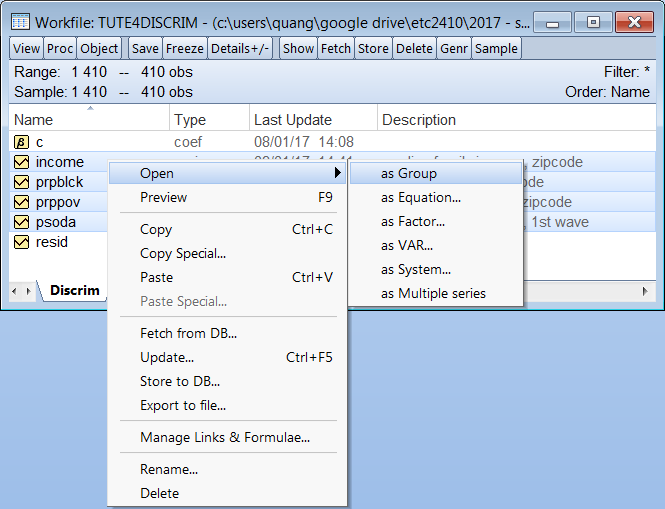
\includegraphics{tute5_1}}
\end{figure}
\vspace{-\baselineskip}
\begin{figure}[H]
	\centerline{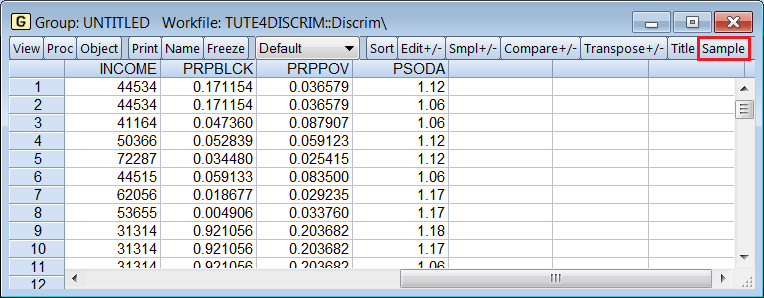
\includegraphics{tute5_2}}
\end{figure}
\vspace{-\baselineskip}
\begin{figure}[H]
	\centerline{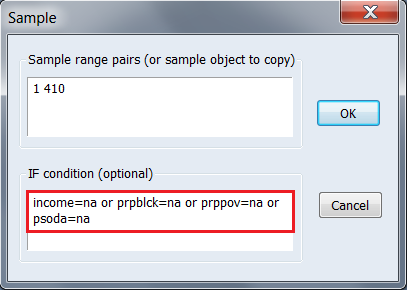
\includegraphics{tute5_3}}
\end{figure}
\vspace{-\baselineskip}
\begin{figure}[H]
	\centerline{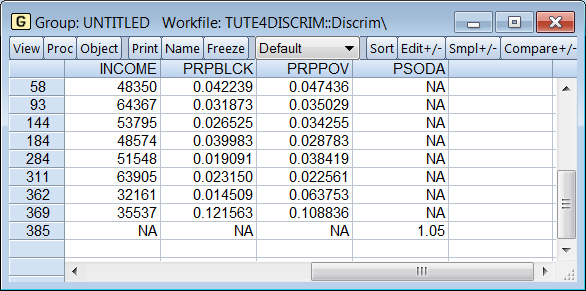
\includegraphics{tute5_4}}
\end{figure}
\vspace{-\baselineskip}
\noindent We can see that the $385^{th}$ district in our sample data set has a missing value for $income$, $prpblck$ and $prppov$. The $58^{th}, 93^{rd}, 144^{th}, 284^{th}, 311^{th},  362^{nd}\ \&\ 369^{th}$ district in our sample data set as a missing value for $psoda$.
\begin{figure}[H]
	\centerline{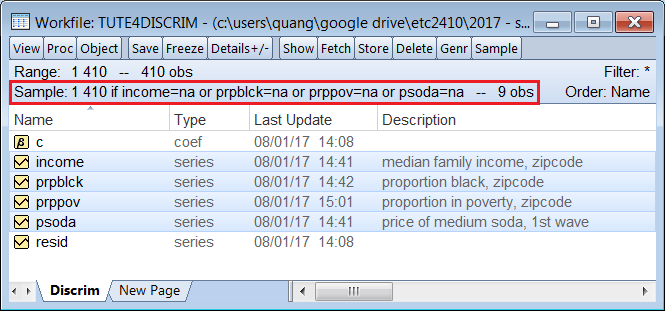
\includegraphics{tute5_5}}
\end{figure}
\vspace{-\baselineskip}
$$(Ensure\ that\ sample\ is\ set\ back\ to\ the\ original\ data\ set) $$
\begin{figure}[H]
	\centerline{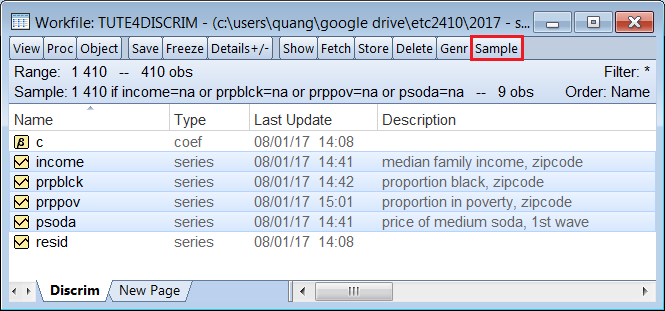
\includegraphics{tute5_6}}
\end{figure}
\vspace{-\baselineskip}
\begin{figure}[H]
	\centerline{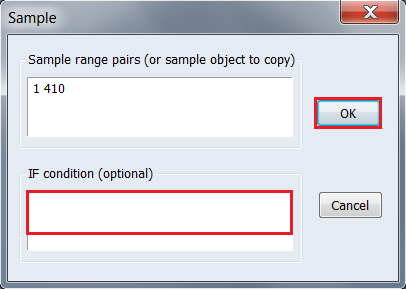
\includegraphics{tute5_7}}
\end{figure}
\vspace{-\baselineskip}
\begin{figure}[H]
	\centerline{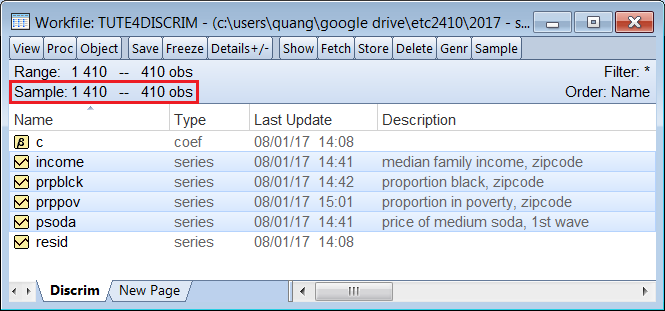
\includegraphics{tute5_8}}
\end{figure}
\vspace{-\baselineskip}

\noindent Because of the missing values in our data set, we should be careful when obtaining summary statistics for a \uline{group of variables}. To obtain summary statistics for the variables the $prpblck$, $income$, $prppov$ and $psoda$ with each variable's \uline{individual sample} in EViews,
$$Quick \to Group\ Statistics \to Descriptive\ Statistics \to \underline{Individual\ Sample}$$
\begin{figure}[H]
	\centerline{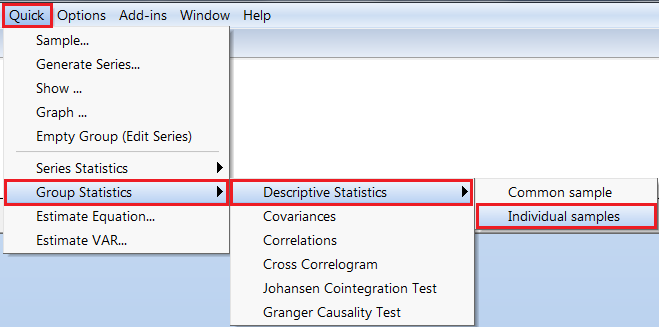
\includegraphics{tute5_9}}
\end{figure}
\vspace{-\baselineskip}
\noindent then type in the variables of interest in the \textit{Series List} dialog box,
\begin{figure}[H]
	\centerline{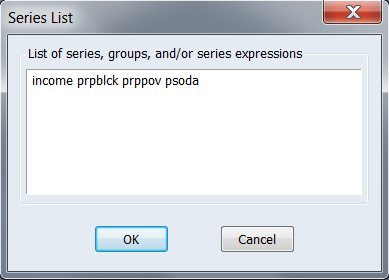
\includegraphics{tute5_10}}
\end{figure}
\vspace{-\baselineskip}
%%%%%%%%%% TABLE OBJECT %%%%%%%%%%
\begin{table}[H]
	\centering
	\begin{tabular}{lrrrr}
		\multicolumn{1}{c}{}&\multicolumn{1}{c}{INCOME}&\multicolumn{1}{c}{PRPBLCK}&\multicolumn{1}{c}{PRPPOV}&\multicolumn{1}{c}{PSODA}\\
		\multicolumn{1}{l}{Mean}&\multicolumn{1}{c}{$47053.78$}&\multicolumn{1}{c}{$0.113486$}&\multicolumn{1}{c}{$0.071297$}&\multicolumn{1}{c}{$1.044876$}\\
		\multicolumn{1}{l}{Median}&\multicolumn{1}{c}{$46272.00$}&\multicolumn{1}{c}{$0.041444$}&\multicolumn{1}{c}{$0.044441$}&\multicolumn{1}{c}{$1.060000$}\\
		\multicolumn{1}{l}{Maximum}&\multicolumn{1}{c}{$136529.0$}&\multicolumn{1}{c}{$0.981658$}&\multicolumn{1}{c}{$0.418480$}&\multicolumn{1}{c}{$1.490000$}\\
		\multicolumn{1}{l}{Minimum}&\multicolumn{1}{c}{$15919.00$}&\multicolumn{1}{c}{$0.000000$}&\multicolumn{1}{c}{$0.004298$}&\multicolumn{1}{c}{$0.730000$}\\
		\multicolumn{1}{l}{Std. Dev.}&\multicolumn{1}{c}{$13179.29$}&\multicolumn{1}{c}{$0.182416$}&\multicolumn{1}{c}{$0.067439$}&\multicolumn{1}{c}{$0.088687$}\\
		\multicolumn{1}{l}{Skewness}&\multicolumn{1}{c}{$0.962831$}&\multicolumn{1}{c}{$2.700012$}&\multicolumn{1}{c}{$2.222999$}&\multicolumn{1}{c}{$0.348905$}\\
		\multicolumn{1}{l}{Kurtosis}&\multicolumn{1}{c}{$7.551386$}&\multicolumn{1}{c}{$10.56841$}&\multicolumn{1}{c}{$8.212019$}&\multicolumn{1}{c}{$4.582298$}\\
		\multicolumn{1}{c}{}&\multicolumn{1}{c}{}&\multicolumn{1}{c}{}&\multicolumn{1}{c}{}&\multicolumn{1}{c}{}\\
		\multicolumn{1}{l}{Jarque-Bera}&\multicolumn{1}{c}{$416.2135$}&\multicolumn{1}{c}{$1473.100$}&\multicolumn{1}{c}{$799.8001$}&\multicolumn{1}{c}{$50.09267$}\\
		\multicolumn{1}{l}{Probability}&\multicolumn{1}{c}{$0.000000$}&\multicolumn{1}{c}{$0.000000$}&\multicolumn{1}{c}{$0.000000$}&\multicolumn{1}{c}{$0.000000$}\\
		\multicolumn{1}{c}{}&\multicolumn{1}{c}{}&\multicolumn{1}{c}{}&\multicolumn{1}{c}{}&\multicolumn{1}{c}{}\\
		\multicolumn{1}{l}{Sum}&\multicolumn{1}{c}{$19244998$}&\multicolumn{1}{c}{$46.41594$}&\multicolumn{1}{c}{$29.16060$}&\multicolumn{1}{c}{$420.0400$}\\
		\multicolumn{1}{l}{Sum Sq. Dev.}&\multicolumn{1}{c}{$7.09E+10$}&\multicolumn{1}{c}{$13.57651$}&\multicolumn{1}{c}{$1.855573$}&\multicolumn{1}{c}{$3.154044$}\\
		\multicolumn{1}{c}{}&\multicolumn{1}{c}{}&\multicolumn{1}{c}{}&\multicolumn{1}{c}{}&\multicolumn{1}{c}{}\\
		\multicolumn{1}{l}{Observations}&\multicolumn{1}{c}{$409$}&\multicolumn{1}{c}{$409$}&\multicolumn{1}{c}{$409$}&\multicolumn{1}{c}{$402$}\\
	\end{tabular}
	\caption{Descriptives statistics of \textit{median family income}, \textit{proportion of the population that is black}, \textit{proportion of the population in poverty} and \textit{price of medium soda} for each variable's individual sample of districts.}
	\label{tbl:desstat}
\end{table}
\vspace{-\baselineskip}

\noindent To obtain summary statistics for the variables the $prpblck$, $income$, $prppov$ and $psoda$ using the $common\ sample$ in EViews,
$$Quick \to Group\ Statistics \to Descriptive\ Statistics \to \underline{Common\ Sample}$$
\begin{figure}[H]
	\centering
	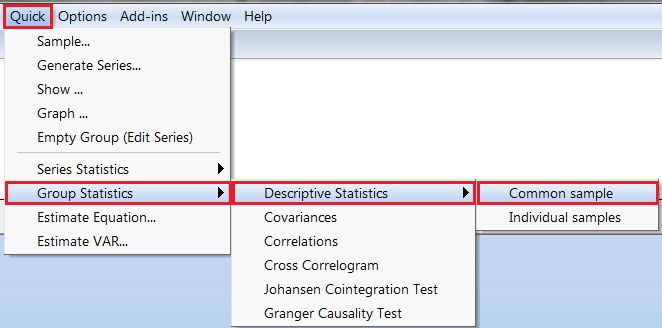
\includegraphics{tute5_29}
\end{figure}
\vspace{-\baselineskip}
\noindent then type in the variables of interest in the \textit{Series List} dialog box,
\begin{figure}[H]
	\centerline{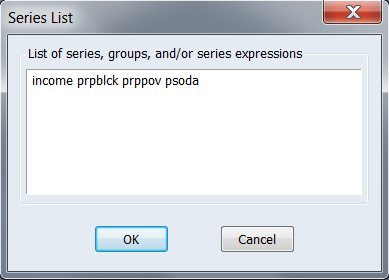
\includegraphics{tute5_10}}
\end{figure}
\vspace{-\baselineskip}
%%%%%%%%%% TABLE OBJECT %%%%%%%%%%
\begin{table}[H]
	\centering
	\begin{tabular}{lrrrr}
		\multicolumn{1}{c}{}&\multicolumn{1}{c}{INCOME}&\multicolumn{1}{c}{PRPBLCK}&\multicolumn{1}{c}{PRPPOV}&\multicolumn{1}{c}{PSODA}\\
		\multicolumn{1}{l}{Mean}&\multicolumn{1}{c}{$46999.40$}&\multicolumn{1}{c}{$0.114955$}&\multicolumn{1}{c}{$0.071774$}&\multicolumn{1}{c}{$1.044863$}\\
		\multicolumn{1}{l}{Median}&\multicolumn{1}{c}{$46255.00$}&\multicolumn{1}{c}{$0.042239$}&\multicolumn{1}{c}{$0.044441$}&\multicolumn{1}{c}{$1.060000$}\\
		\multicolumn{1}{l}{Maximum}&\multicolumn{1}{c}{$136529.0$}&\multicolumn{1}{c}{$0.981658$}&\multicolumn{1}{c}{$0.418480$}&\multicolumn{1}{c}{$1.490000$}\\
		\multicolumn{1}{l}{Minimum}&\multicolumn{1}{c}{$15919.00$}&\multicolumn{1}{c}{$0.000000$}&\multicolumn{1}{c}{$0.004298$}&\multicolumn{1}{c}{$0.730000$}\\
		\multicolumn{1}{l}{Std. Dev.}&\multicolumn{1}{c}{$13215.33$}&\multicolumn{1}{c}{$0.183875$}&\multicolumn{1}{c}{$0.067924$}&\multicolumn{1}{c}{$0.088798$}\\
		\multicolumn{1}{l}{Skewness}&\multicolumn{1}{c}{$0.980441$}&\multicolumn{1}{c}{$2.666880$}&\multicolumn{1}{c}{$2.200406$}&\multicolumn{1}{c}{$0.348907$}\\
		\multicolumn{1}{l}{Kurtosis}&\multicolumn{1}{c}{$7.615445$}&\multicolumn{1}{c}{$10.35573$}&\multicolumn{1}{c}{$8.075490$}&\multicolumn{1}{c}{$4.571177$}\\
		\multicolumn{1}{c}{}&\multicolumn{1}{c}{}&\multicolumn{1}{c}{}&\multicolumn{1}{c}{}&\multicolumn{1}{c}{}\\
		\multicolumn{1}{l}{Jarque-Bera}&\multicolumn{1}{c}{$420.1710$}&\multicolumn{1}{c}{$1379.368$}&\multicolumn{1}{c}{$754.0096$}&\multicolumn{1}{c}{$49.38217$}\\
		\multicolumn{1}{l}{Probability}&\multicolumn{1}{c}{$0.000000$}&\multicolumn{1}{c}{$0.000000$}&\multicolumn{1}{c}{$0.000000$}&\multicolumn{1}{c}{$0.000000$}\\
		\multicolumn{1}{c}{}&\multicolumn{1}{c}{}&\multicolumn{1}{c}{}&\multicolumn{1}{c}{}&\multicolumn{1}{c}{}\\
		\multicolumn{1}{l}{Sum}&\multicolumn{1}{c}{$18846761$}&\multicolumn{1}{c}{$46.09700$}&\multicolumn{1}{c}{$28.78153$}&\multicolumn{1}{c}{$418.9900$}\\
		\multicolumn{1}{l}{Sum Sq. Dev.}&\multicolumn{1}{c}{$6.99E+10$}&\multicolumn{1}{c}{$13.52401$}&\multicolumn{1}{c}{$1.845495$}&\multicolumn{1}{c}{$3.154017$}\\
		\multicolumn{1}{c}{}&\multicolumn{1}{c}{}&\multicolumn{1}{c}{}&\multicolumn{1}{c}{}&\multicolumn{1}{c}{}\\
		\multicolumn{1}{l}{Observations}&\multicolumn{1}{c}{$401$}&\multicolumn{1}{c}{$401$}&\multicolumn{1}{c}{$401$}&\multicolumn{1}{c}{$401$}\\
	\end{tabular}
	\caption{Descriptives statistics of \textit{median family income}, \textit{proportion of the population that is black}, \textit{proportion of the population in poverty} and \textit{price of medium soda} using a common sample.}
	%\label{tab:}
\end{table}
\vspace{-\baselineskip}
\noindent \textcolor{red}
{
	\ul{(ii) Consider a model to explain the price of soda in a district, $psoda$ in terms of the proportion of the population that is black in a district ($prpblck$) and the median income in a district ($income$)} $$psoda = \beta_0 + \beta_1prpblck + \beta_2income + u$$ Estimate this model by OLS and report the results in equation form, including the sample size and $R^2$. (Do not use scientific notation when reporting the estimates.)
}

\noindent To estimate this model in EViews,
$$Quick \to Estimate\ Equation$$
\begin{figure}[H]
	\centering
	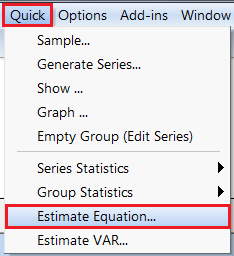
\includegraphics{tute5_11}
\end{figure}
\vspace{-\baselineskip}
\noindent then in the \textit{Equation Estimation} dialog box type in,
$$psoda\ c\ prpblck\ income$$
\begin{figure}[H]
	\centering
	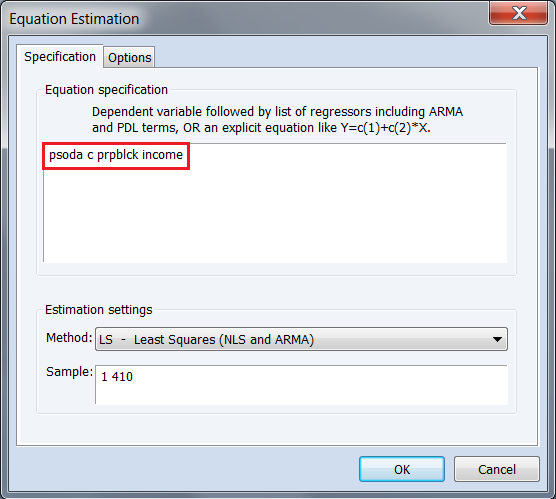
\includegraphics{tute5_12}
\end{figure}
\vspace{-\baselineskip}
\noindent To name (save) the estimated equation,
$$Name \to Name\ to\ identify\ object: eq01$$
$$(This\ names\ the\ equation\ \textit{\textbf{eq01}})$$
\begin{figure}[H]
	\centering
	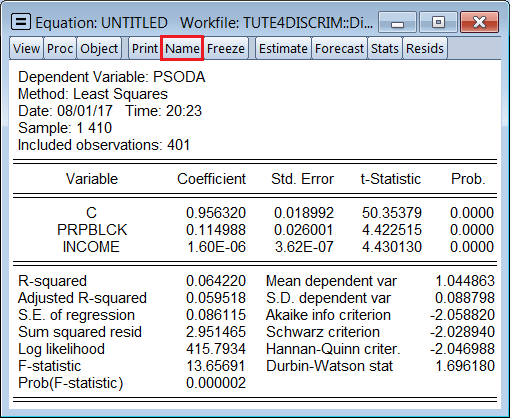
\includegraphics{tute5_13}
\end{figure}
\vspace{-\baselineskip}
\begin{figure}[H]
	\centering
	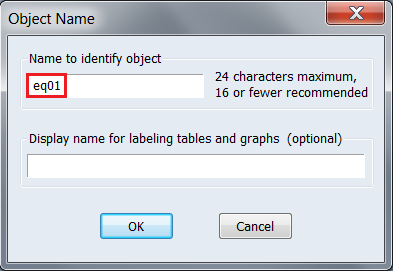
\includegraphics{tute5_14}
\end{figure}
\vspace{-\baselineskip}

\noindent The estimated model,
$$\widehat{psoda} = \hat{\beta}_0 + \hat{\beta}_1prpblck + \hat{\beta}_2income$$
\noindent \textcolor{red}
{
	Interpret the coefficient on $prpblck$ (with a 0.1 increase in $prpblck$)
}

\noindent $\hat{\beta}_1 = 0.1150$

\noindent The model estimates that for a 0.1 increase in the proportion of blacks in a district i.e. a 10 percentage-point increase (not a 10 percent increase), the price of soda in that district will increase by $0.1150\times0.1=0.0115$ i.e. \$0.0115 or about 1.2 cents, on average, holding median family income constant.

\noindent \textcolor{red}
{
	Is $\hat{\beta}_1 = 0.1150$ economically large?
}

\noindent Although a 1.2 cent increase in soda price for a 0.1 increase in the proportion of the population in a district that is black, holding median family income constant, does not seem large, if we compare the soda price between districts with and without a black population, holding median family income constant, we find that the difference is 11.50 cent,
$${\Delta}income = 0$$
$${\Delta}prpblck = 1$$
\begin{align*}
{\Delta}\widehat{psoda} &= \hat{\beta}_1{\Delta}prpblck + \hat{\beta}_2{\Delta}income \\
&= \hat{\beta}_1\times1 \\
&= 0.1150
\end{align*}
\noindent Whether this is large depends on the average soda price. From our sample of districts, the average soda price was \$1.04 so an \$11.5 cent difference would seem large.

\noindent \textcolor{red}
{
	(iv) Reporting estimated models and rescaling
}

\noindent Data initially obtained may not be in a convenient scale for regression analysis. In our example, $psoda$ and $income$ are both is measured in dollars and we obtained the following estimated model,
$$\widehat{psoda} = $$

\noindent The interpretation of the estimated coefficient of income,

\centering 
\textit{When a district’s median family income increases by \$1, we estimate that the price of soda in that district will increase by \$0.00000016, holding district's proportion of the population that is black constant.}
\justify
Although nothing is mathematically wrong with this, it leads to a discussion of changes that are so small as to seem irrelevant. 
By changing the unit of measurement of $psoda$ to cent, we obtain the following estimated model,
%%%%%%%%%% TABLE OBJECT %%%%%%%%%%
\begin{table}[H]
	\centering
	\begin{tabular}{lrrrr}
		\multicolumn{4}{l}{Dependent Variable: PSODA\_CENT}&\multicolumn{1}{c}{}\\
		\multicolumn{3}{l}{Method: Least Squares}&\multicolumn{1}{c}{}&\multicolumn{1}{c}{}\\
		\multicolumn{3}{l}{Date: 08/12/17   Time: 16:08}&\multicolumn{1}{c}{}&\multicolumn{1}{c}{}\\
		\multicolumn{2}{l}{Sample: 1 410}&\multicolumn{1}{c}{}&\multicolumn{1}{c}{}&\multicolumn{1}{c}{}\\
		\multicolumn{3}{l}{Included observations: 401}&\multicolumn{1}{c}{}&\multicolumn{1}{c}{}\\
		[4.5pt] \hline \\ [-4.5pt]
		\multicolumn{1}{c}{Variable}&\multicolumn{1}{r}{Coefficient}&\multicolumn{1}{r}{Std. Error}&\multicolumn{1}{r}{t-Statistic}&\multicolumn{1}{r}{Prob.}\\
		[4.5pt] \hline \\ [-4.5pt]
		\multicolumn{1}{c}{C}&\multicolumn{1}{r}{$95.63197$}&\multicolumn{1}{r}{$1.899201$}&\multicolumn{1}{r}{$50.35379$}&\multicolumn{1}{r}{$0.0000$}\\
		\multicolumn{1}{c}{PRPBLCK}&\multicolumn{1}{r}{$11.49882$}&\multicolumn{1}{r}{$2.600064$}&\multicolumn{1}{r}{$4.422515$}&\multicolumn{1}{r}{$0.0000$}\\
		\multicolumn{1}{c}{INCOME}&\multicolumn{1}{r}{$0.000160$}&\multicolumn{1}{r}{$3.62E-05$}&\multicolumn{1}{r}{$4.430130$}&\multicolumn{1}{r}{$0.0000$}\\
		[4.5pt] \hline \\ [-4.5pt]
		\multicolumn{1}{l}{R-squared}&\multicolumn{1}{r}{$0.064220$}&\multicolumn{2}{l}{Mean dependent var}&\multicolumn{1}{r}{$104.4863$}\\
		\multicolumn{1}{l}{Adjusted R-squared}&\multicolumn{1}{r}{$0.059518$}&\multicolumn{2}{l}{S.D. dependent var}&\multicolumn{1}{r}{$8.879777$}\\
		\multicolumn{1}{l}{S.E. of regression}&\multicolumn{1}{r}{$8.611470$}&\multicolumn{2}{l}{Akaike info criterion}&\multicolumn{1}{r}{$7.151520$}\\
		\multicolumn{1}{l}{Sum squared resid}&\multicolumn{1}{r}{$29514.65$}&\multicolumn{2}{l}{Schwarz criterion}&\multicolumn{1}{r}{$7.181400$}\\
		\multicolumn{1}{l}{Log likelihood}&\multicolumn{1}{r}{$-1430.880$}&\multicolumn{2}{l}{Hannan-Quinn criter.}&\multicolumn{1}{r}{$7.163352$}\\
		\multicolumn{1}{l}{F-statistic}&\multicolumn{1}{r}{$13.65691$}&\multicolumn{2}{l}{Durbin-Watson stat}&\multicolumn{1}{r}{$1.696180$}\\
		\multicolumn{1}{l}{Prob(F-statistic)}&\multicolumn{1}{r}{$0.000002$}&\multicolumn{1}{c}{}&\multicolumn{1}{c}{}&\multicolumn{1}{c}{}\\
		[4.5pt] \hline \\ [-4.5pt]
	\end{tabular}
	\caption{Regression output of the \textit{price of soda in cents} on a constant, the \textit{proportion of the population that is black} and \textit{median family income in \$}.}
	%\label{tab:}
\end{table}
\vspace{-\baselineskip}
$$\widehat{psoda\_cent} = $$
\noindent and the interpretation of the estimated coefficient of $income$ becomes,

\centering
\textit{When a district’s median family income increases by \$1, we estimate that the price of soda in that district increases by 0.00016 cent, holding the proportion of the population that is black in a district constant.}

\justify
\noindent When the price of soda is rescaled from dollars to cents we do so by multiplying the original variable $psoda$ by $100$,
$$psoda\_cent = 100psoda$$
and the estimated coefficients will rescale according,
\begin{align*}
\hat{\beta}_{0}^{*} &= 100\hat{\beta}_{0} \\
\hat{\beta}_{1}^{*} &= 100\hat{\beta}_{1} \\
\hat{\beta}_{2}^{*} &= 100\hat{\beta}_{2}
\end{align*}
\noindent where,
\begin{align*}
\widehat{psoda} &= \hat{\beta}_0 + \hat{\beta}_1prpblck + \hat{\beta}_2income \\
\widehat{psoda\_cent} &= 100\hat{\beta}_0 + 100\hat{\beta}_1prpblck + 100\hat{\beta}_2income \\
\widehat{psoda\_cent} &= \hat{\beta}_{0}^{*} + \hat{\beta}_{1}^{*}prpblck + \hat{\beta}_{2}^{*}income
\end{align*}
\noindent If we also rescale median family income from dollars to \$'000, we obtain the following estimated model, $$\widehat{psoda\_cent} = \hat{\beta}_{0}^{*} + \hat{\beta}_{1}^{*}prpblck + 1000\hat{\beta}_{2}^{*}income\_thousand$$
%%%%%%%%%% TABLE OBJECT %%%%%%%%%%
\begin{table}[H]
	\centering
	\begin{tabular}{lrrrr}
		\multicolumn{4}{l}{Dependent Variable: PSODA\_CENT}&\multicolumn{1}{c}{}\\
		\multicolumn{3}{l}{Method: Least Squares}&\multicolumn{1}{c}{}&\multicolumn{1}{c}{}\\
		\multicolumn{3}{l}{Date: 08/12/17   Time: 16:28}&\multicolumn{1}{c}{}&\multicolumn{1}{c}{}\\
		\multicolumn{2}{l}{Sample: 1 410}&\multicolumn{1}{c}{}&\multicolumn{1}{c}{}&\multicolumn{1}{c}{}\\
		\multicolumn{3}{l}{Included observations: 401}&\multicolumn{1}{c}{}&\multicolumn{1}{c}{}\\
		[4.5pt] \hline \\ [-4.5pt]
		\multicolumn{1}{c}{Variable}&\multicolumn{1}{r}{Coefficient}&\multicolumn{1}{r}{Std. Error}&\multicolumn{1}{r}{t-Statistic}&\multicolumn{1}{r}{Prob.}\\
		[4.5pt] \hline \\ [-4.5pt]
		\multicolumn{1}{c}{C}&\multicolumn{1}{r}{$95.63197$}&\multicolumn{1}{r}{$1.899201$}&\multicolumn{1}{r}{$50.35379$}&\multicolumn{1}{r}{$0.0000$}\\
		\multicolumn{1}{c}{PRPBLCK}&\multicolumn{1}{r}{$11.49882$}&\multicolumn{1}{r}{$2.600064$}&\multicolumn{1}{r}{$4.422515$}&\multicolumn{1}{r}{$0.0000$}\\
		\multicolumn{1}{c}{INCOME\_THOUSAND}&\multicolumn{1}{r}{$0.160267$}&\multicolumn{1}{r}{$0.036177$}&\multicolumn{1}{r}{$4.430130$}&\multicolumn{1}{r}{$0.0000$}\\
		[4.5pt] \hline \\ [-4.5pt]
		\multicolumn{1}{l}{R-squared}&\multicolumn{1}{r}{$0.064220$}&\multicolumn{2}{l}{Mean dependent var}&\multicolumn{1}{r}{$104.4863$}\\
		\multicolumn{1}{l}{Adjusted R-squared}&\multicolumn{1}{r}{$0.059518$}&\multicolumn{2}{l}{S.D. dependent var}&\multicolumn{1}{r}{$8.879777$}\\
		\multicolumn{1}{l}{S.E. of regression}&\multicolumn{1}{r}{$8.611470$}&\multicolumn{2}{l}{Akaike info criterion}&\multicolumn{1}{r}{$7.151520$}\\
		\multicolumn{1}{l}{Sum squared resid}&\multicolumn{1}{r}{$29514.65$}&\multicolumn{2}{l}{Schwarz criterion}&\multicolumn{1}{r}{$7.181400$}\\
		\multicolumn{1}{l}{Log likelihood}&\multicolumn{1}{r}{$-1430.880$}&\multicolumn{2}{l}{Hannan-Quinn criter.}&\multicolumn{1}{r}{$7.163352$}\\
		\multicolumn{1}{l}{F-statistic}&\multicolumn{1}{r}{$13.65691$}&\multicolumn{2}{l}{Durbin-Watson stat}&\multicolumn{1}{r}{$1.696180$}\\
		\multicolumn{1}{l}{Prob(F-statistic)}&\multicolumn{1}{r}{$0.000002$}&\multicolumn{1}{c}{}&\multicolumn{1}{c}{}&\multicolumn{1}{c}{}\\
		[4.5pt] \hline \\ [-4.5pt]
	\end{tabular}
	\caption{Regression output of the \textit{price of soda in cents} on a constant, the \textit{proportion of the population that is black} and \textit{median family income in \$'000}.}
	%\label{tab:}
\end{table}

\vspace{-\baselineskip}
$$\widehat{psoda\_cent}=$$
\noindent which provides a more meaningful interpretation,

\centering
\textit{When a district’s median family income increases by \$1,000, the model estimates that the price of soda in that district will increase by 0.16 cents, holding the proportion of the population that is black in a district constant.}

\justify
\noindent And if we also express $prpblck$ in percentage points, $$prpblck\% = 100\times prpblck$$ $$\widehat{psoda\_cent} = \hat{\beta}_{0}^{*} + \dfrac{1}{1000}\hat{\beta}_{1}^{*}prpblck\% + 1000\hat{\beta}_{2}^{*}income\_thousand$$

\justify
\noindent As we can see, the data has been rescaled without changing the real underlying relationship between the price of soda and median family income. The interpretation remains mathematically correct and the magnitudes are more relevant and easy for discussion.

\noindent \textcolor{red}
{
	\ul{(iii) Compare the estimate from part (ii) with the simple regression estimate from $psoda$ on $prpblck$. Is the discrimination effect larger or smaller when you control for $income$?}
}

\noindent To estimate this model in EViews,
$$Quick \to Estimate\ Equation$$
\begin{figure}[H]
	\centering
	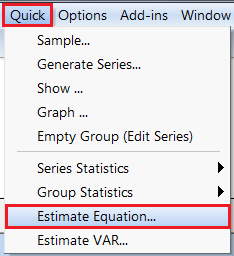
\includegraphics{tute5_11}
\end{figure}
\vspace{-\baselineskip}
\noindent then in the \textit{Equation Estimation} dialog box type in,
$$psoda\ c\ prpblck$$
\begin{figure}[H]
	\centering
	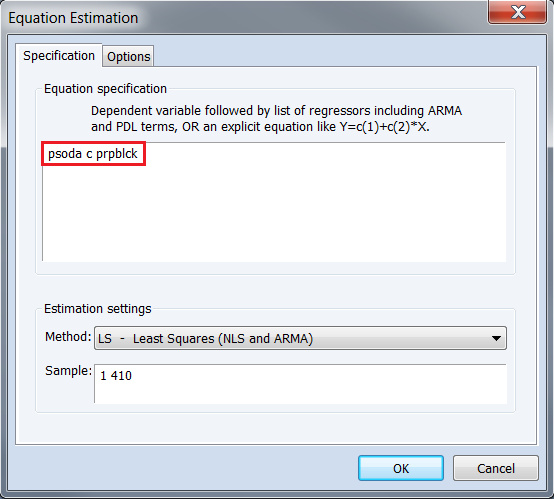
\includegraphics{tute5_16}
\end{figure}
\vspace{-\baselineskip}
%%%%%%%%%% TABLE OBJECT %%%%%%%%%%
\begin{table}[H]
	\centering
	\begin{tabular}{lrrrr}
		\multicolumn{3}{l}{Dependent Variable: PSODA}&\multicolumn{1}{c}{}&\multicolumn{1}{c}{}\\
		\multicolumn{3}{l}{Method: Least Squares}&\multicolumn{1}{c}{}&\multicolumn{1}{c}{}\\
		\multicolumn{3}{l}{Date: 08/12/17   Time: 17:14}&\multicolumn{1}{c}{}&\multicolumn{1}{c}{}\\
		\multicolumn{2}{l}{Sample: 1 410}&\multicolumn{1}{c}{}&\multicolumn{1}{c}{}&\multicolumn{1}{c}{}\\
		\multicolumn{3}{l}{Included observations: 401}&\multicolumn{1}{c}{}&\multicolumn{1}{c}{}\\
		[4.5pt] \hline \\ [-4.5pt]
		\multicolumn{1}{c}{Variable}&\multicolumn{1}{r}{Coefficient}&\multicolumn{1}{r}{Std. Error}&\multicolumn{1}{r}{t-Statistic}&\multicolumn{1}{r}{Prob.}\\
		[4.5pt] \hline \\ [-4.5pt]
		\multicolumn{1}{c}{C}&\multicolumn{1}{r}{$1.037399$}&\multicolumn{1}{r}{$0.005190$}&\multicolumn{1}{r}{$199.8668$}&\multicolumn{1}{r}{$0.0000$}\\
		\multicolumn{1}{c}{PRPBLCK}&\multicolumn{1}{r}{$0.064927$}&\multicolumn{1}{r}{$0.023957$}&\multicolumn{1}{r}{$2.710146$}&\multicolumn{1}{r}{$0.0070$}\\
		[4.5pt] \hline \\ [-4.5pt]
		\multicolumn{1}{l}{R-squared}&\multicolumn{1}{r}{$0.018076$}&\multicolumn{2}{l}{Mean dependent var}&\multicolumn{1}{r}{$1.044863$}\\
		\multicolumn{1}{l}{Adjusted R-squared}&\multicolumn{1}{r}{$0.015615$}&\multicolumn{2}{l}{S.D. dependent var}&\multicolumn{1}{r}{$0.088798$}\\
		\multicolumn{1}{l}{S.E. of regression}&\multicolumn{1}{r}{$0.088102$}&\multicolumn{2}{l}{Akaike info criterion}&\multicolumn{1}{r}{$-2.015673$}\\
		\multicolumn{1}{l}{Sum squared resid}&\multicolumn{1}{r}{$3.097007$}&\multicolumn{2}{l}{Schwarz criterion}&\multicolumn{1}{r}{$-1.995753$}\\
		\multicolumn{1}{l}{Log likelihood}&\multicolumn{1}{r}{$406.1425$}&\multicolumn{2}{l}{Hannan-Quinn criter.}&\multicolumn{1}{r}{$-2.007785$}\\
		\multicolumn{1}{l}{F-statistic}&\multicolumn{1}{r}{$7.344894$}&\multicolumn{2}{l}{Durbin-Watson stat}&\multicolumn{1}{r}{$1.611081$}\\
		\multicolumn{1}{l}{Prob(F-statistic)}&\multicolumn{1}{r}{$0.007015$}&\multicolumn{1}{c}{}&\multicolumn{1}{c}{}&\multicolumn{1}{c}{}\\
		[4.5pt] \hline \\ [-4.5pt]
	\end{tabular}
	\caption{Regression output of $psoda$ on a constant and $prpblck$.}
	%\label{tab:}
\end{table}

\vspace{-\baselineskip}
$$\widehat{psoda}=$$

\noindent The discrimination effect is larger then we control for median family income. For our estimated simple and multiple regression model (not controlling then controlling median family income),
$$\widehat{psoda} = \hat{\alpha}_0 + \hat{\alpha}_1prpblck$$
$$\widehat{psoda} = \hat{\beta}_0 + \hat{\beta}_1prpblck + \hat{\beta}_2income$$

\noindent $\hat{\alpha}_1$ and $\hat{\beta}_1$ have the following algebraic relationship,
$$\hat{\alpha}_1 = \hat{\beta}_1 + \hat{\beta}_2\hat{\delta}_1$$
\noindent where $\hat{\delta}_1$ is the estimated slope of coefficient of $income$ regressed on a constant and $prpblck$,
$$\widehat{income} = \hat{\delta}_0 + \hat{\delta}_1 prpblck$$
$$\widehat{income} = \underset{(692.7061)}{50608.36} - \underset{(3227.179)}{31321.63} prpblck$$

%%%%%%%%%% TABLE OBJECT %%%%%%%%%%
\begin{table}[H]
	\centering
	\begin{tabular}{lrrrr}
		\multicolumn{3}{l}{Dependent Variable: INCOME}&\multicolumn{1}{c}{}&\multicolumn{1}{c}{}\\
		\multicolumn{3}{l}{Method: Least Squares}&\multicolumn{1}{c}{}&\multicolumn{1}{c}{}\\
		\multicolumn{3}{l}{Date: 08/13/17   Time: 05:02}&\multicolumn{1}{c}{}&\multicolumn{1}{c}{}\\
		\multicolumn{2}{l}{Sample: 1 410}&\multicolumn{1}{c}{}&\multicolumn{1}{c}{}&\multicolumn{1}{c}{}\\
		\multicolumn{3}{l}{Included observations: 409}&\multicolumn{1}{c}{}&\multicolumn{1}{c}{}\\
		[4.5pt] \hline \\ [-4.5pt]
		\multicolumn{1}{c}{Variable}&\multicolumn{1}{r}{Coefficient}&\multicolumn{1}{r}{Std. Error}&\multicolumn{1}{r}{t-Statistic}&\multicolumn{1}{r}{Prob.}\\
		[4.5pt] \hline \\ [-4.5pt]
		\multicolumn{1}{c}{C}&\multicolumn{1}{r}{$50608.36$}&\multicolumn{1}{r}{$692.7061$}&\multicolumn{1}{r}{$73.05892$}&\multicolumn{1}{r}{$0.0000$}\\
		\multicolumn{1}{c}{PRPBLCK}&\multicolumn{1}{r}{$-31321.63$}&\multicolumn{1}{r}{$3227.179$}&\multicolumn{1}{r}{$-9.705576$}&\multicolumn{1}{r}{$0.0000$}\\
		[4.5pt] \hline \\ [-4.5pt]
		\multicolumn{1}{l}{R-squared}&\multicolumn{1}{r}{$0.187946$}&\multicolumn{2}{l}{Mean dependent var}&\multicolumn{1}{r}{$47053.78$}\\
		\multicolumn{1}{l}{Adjusted R-squared}&\multicolumn{1}{r}{$0.185951$}&\multicolumn{2}{l}{S.D. dependent var}&\multicolumn{1}{r}{$13179.29$}\\
		\multicolumn{1}{l}{S.E. of regression}&\multicolumn{1}{r}{$11890.97$}&\multicolumn{2}{l}{Akaike info criterion}&\multicolumn{1}{r}{$21.60982$}\\
		\multicolumn{1}{l}{Sum squared resid}&\multicolumn{1}{r}{$5.75E+10$}&\multicolumn{2}{l}{Schwarz criterion}&\multicolumn{1}{r}{$21.62945$}\\
		\multicolumn{1}{l}{Log likelihood}&\multicolumn{1}{r}{$-4417.209$}&\multicolumn{2}{l}{Hannan-Quinn criter.}&\multicolumn{1}{r}{$21.61759$}\\
		\multicolumn{1}{l}{F-statistic}&\multicolumn{1}{r}{$94.19820$}&\multicolumn{2}{l}{Durbin-Watson stat}&\multicolumn{1}{r}{$1.035961$}\\
		\multicolumn{1}{l}{Prob(F-statistic)}&\multicolumn{1}{r}{$0.000000$}&\multicolumn{1}{c}{}&\multicolumn{1}{c}{}&\multicolumn{1}{c}{}\\
		[4.5pt] \hline \\ [-4.5pt]
	\end{tabular}
	\caption{Regression output of $income$ on a constant and $prpblck$.}
	%\label{tab:}
\end{table}



\end{document}
